\chapter{绪论} 
\section{研究背景与相关工作}
\subsection{非线性偏微分方程精确解的研究背景与相关工作}
\subsection{非线性差分方程精确解的研究背景与相关工作}
\section{本文的选题和主要工作}
本文的主要工作分为非线性微分方程求解\zdh 非线性差分方程求解和非线性积分化简三个部分, 它们的逻辑结构如\reffig{outline}所示. 在\reffig{outline}中, 椭圆表示方法\zdh 矩形表示软件包. 其中, 软件包元素的第一行是软件包的名称, 第二行是软件包用途的简要说明. 软件包以4种颜色进行区分, 黄色表示基础工具, 蓝色表示用于求解差分方程, 绿色表示用于求解微分方程, 粉色表示用于进行积分化简. 即, 对于微分\zdh 差分\zdh 积分这三种不同的非线性系统的一些具体问题, 本文共实现了8个Maple软件包.

\begin{figure}[htbp]
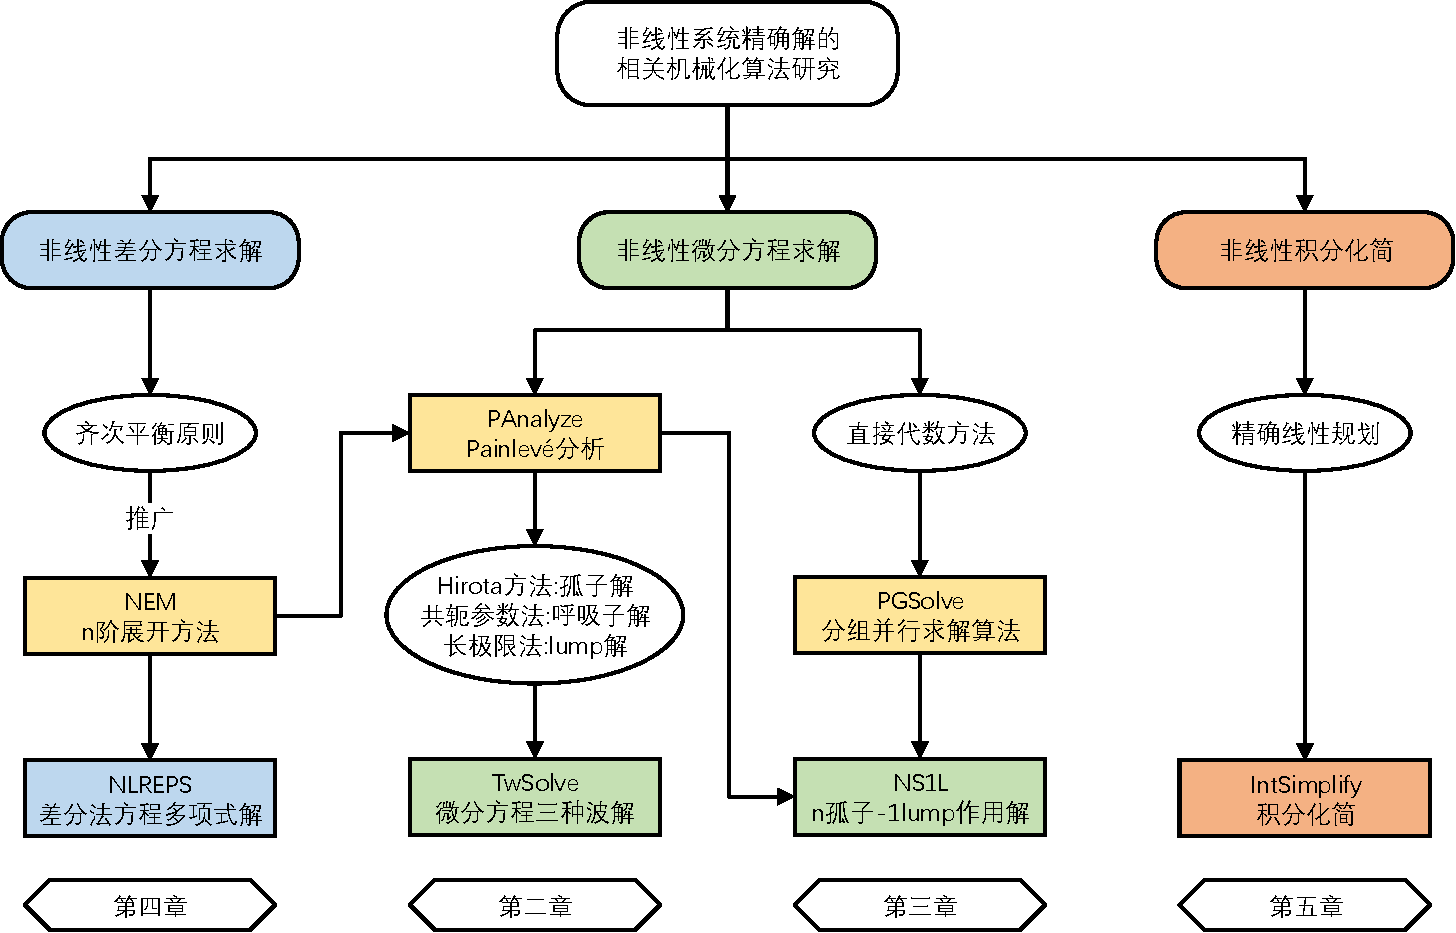
\includegraphics[width=\textwidth]{fig/outline.pdf}
\caption{本文工作大纲图}\label{outline}
\end{figure}

在第二章中, 本文以 \Painleve{} 分析和简单 Hirota 方法为基础, 实现了非线性演化方程三种波解的求解. 其中, 孤子解通过简单 Hirota 方法获得. 获得孤子解之后, 可以通过共轭参数法得到呼吸子解, 通过长极限法得到LUMP解. 本文将上述求解过程打包在TwSolver软件包中.

直接代数方法在微分方程求解中也有广泛的应用, 但其往往伴随着大规模代数方程组的求解. 在第三章中, 本文针对大规模代数方程组求解困难的问题, 设计了一个分组并行求解的算法, 并将其实现为 PGSolve 软件包. 作为PGSolve的应用实例, 本文开发了用直接代数方法求$n$-孤子和1-LUMP相互作用解的软件包 NS1L. 

在第四章中, 受到在微分方程求解中被广泛应用的齐次平衡原则的启发, 本文将其用于求解非线性差分方程的多项式解. 齐次平衡原则通过平衡方程中最高次项的次数来确定解的次数, 只能在一些情况下生效. 本文考虑同时平衡方程中最高$n$项的次数和系数, 提出了$n$阶展开方法来处理齐次平衡原则不能处理的情况, 并将其实现为一个便于拓展应用的软件包 NEM. 基于NEM, 实现了能够求解非线性差分方程所有多项式解的软件包 NLREPS. 

在微分方程的求解中, NEM 能够快速地完善基于齐次平衡原则的求解算法. 在第五章中, 我们以双曲正切方法为例, 基于NEM重新实现了一个NTCM软件包. 该软件包在将双曲正切方法推广到$n+1$维的同时, 利用NEM在阶数分析上的优势, 求解了许多以往不能求解的方程. 同时, 我们也以 \Painleve{} 分析为例展示了 NEM 的作用. 

在第六章中, 因为在非线性微分方程求解的过程中往往需要进行非线性积分表达式的化简, 本文将非线性积分化简作为一个具有挑战性的任务进行研究. 首先, 本文建立了一个代数系统将关于抽象函数的积分多项式视为标准积分项的线性组合. 然后, 基于导数的乘法规则, 设计了一个递归算法来寻找所有的二项合并规则. 最后, 基于这些规则将化简问题转化为一个精确线性规划问题进行求解, 实现了非线性积分表达式化简的软件包 IntSimplify. 

第七章对本文完成的工作进行了总结与讨论,概括了本文的主要研究方法和结论,并提出了对未来工作的展望.
